% Problem statement
% latest link for robocup@work dataset

\documentclass[rnd]{mas_proposal}
\usepackage[utf8]{inputenc}
\usepackage{amsmath}
\usepackage{amsfonts}
\usepackage{amssymb}
\usepackage{graphicx}
\usepackage{float}
\usepackage{array}

\title{Uncertainty Estimation for Quantized Deep Learning Models: Comparative Study}

%Footer title in line 198 of mas_proposal.cls file
\author{Mohan Raj Nadarajan}
\supervisors{Prof. Dr. Sebastian Houben\\M.Sc. Deebul Sivarajan Nair}
\date{December 2022}


\begin{document}
\maketitle
\pagestyle{plain}
\section{Introduction}
The effectiveness of image processing deep learning models over other conventional machine learning models is indisputable. Though the deep learning models  exhibits higher accuracy, the wrong predictions are with higher value of confidence, which will not only fail the task-but also put human lives at jeopardy in the case of safety critical and real world applications\cite{gawlikowski2021survey}. As a result, it is very important for the deep learning models to be aware of confidence in its prediction, alternatively the uncertainty in its prediction .
\begin{figure}[h!]
    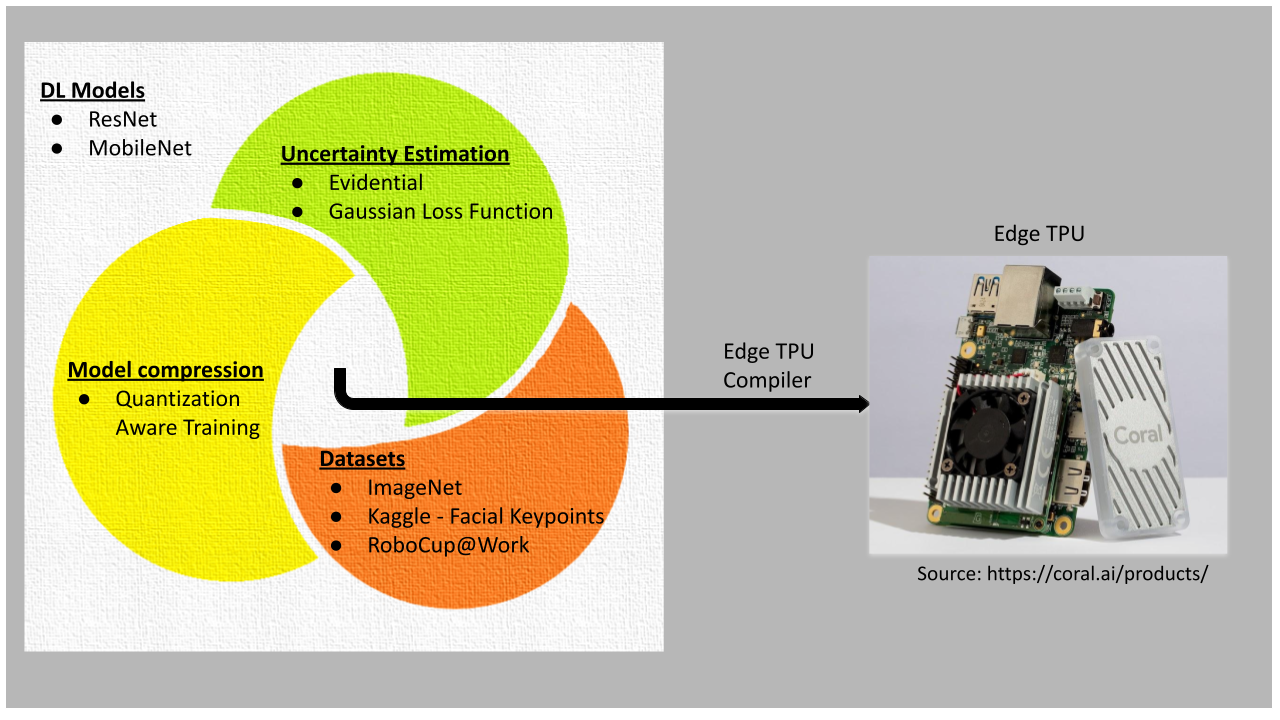
\includegraphics[width=\textwidth]{images/VennDiagram_V4.png}
    \caption{Project components}
    \label{fig:myfigure}
\end{figure}
\\
The predictive uncertainty in a deep learning model is of two types: Aleatoric uncertainty and Epistemic uncertainty or a combination of both\cite{ue_qunatification}. Aleatoric uncertainty also known as data uncertainty is due to the noise in the training data. Epistemic uncertainty also known as model uncertainty is due to uncertainty in the parameters of the model. The epistemic type of uncertainty can be reduced by adding more input data to the model. The deep learning community has provided different uncertainty estimation methods like Monte Carlo dropout\cite{gal2016dropout}, stochastic batch normalization\cite{atanov2018uncertainty}, test-time data augmentation\cite{ayhan2018test}, deep ensembles\cite{lakshminarayanan2017simple}, selective classification\cite{geifman2017selective}, deterministic\cite{abs-2003-02037} and evidential\cite{DBLP:journals/corr/abs-1806-01768} approaches.
\\\\
The state-of-the-art uncertainty estimation methods are mainly proposed for GPU based inference and there does not exist much research on uncertainty estimation in deep learning models for edge devices. Edge AI combines artificial intelligence and edge computing. The advancement in edge devices for AI applications to make real-time insights along with improved privacy, reduced latency and high availability are revolutionizing the world's largest industries and expanding business outcomes across all sectors. Edge AI runs on a wide range of hardware from micro-controller to tensor processing devices for real world applications like smart watches, autonomous cars, mobile phones.
\\\\
Training or inferencing the neural network algorithms on general purpose hardware like CPU (von Neumann architecture) or GPU is inefficient due to higher number of multiply-accumulate operations\cite{hubara2017quantized}. One way to accelerate neural network workload is using the specialized matrix processor called Tensor Processing Unit. They are of domain specific hardware architecture for deep learning and is a combination of matrix multiplication unit (MXU), vector processing unit and high-bandwidth memory. The MXU contains series of multiply-accumulators, connected directly to each other forming a systolic array architecture. This R\&D works evaluates the uncertainty estimation for deep learning models deployed on the Device Under Test(DUT) such as Google Coral - USB accelerator and OAK-D, driven by Intel Movidius Myriad X VPU.
\begin{figure}[h!]
    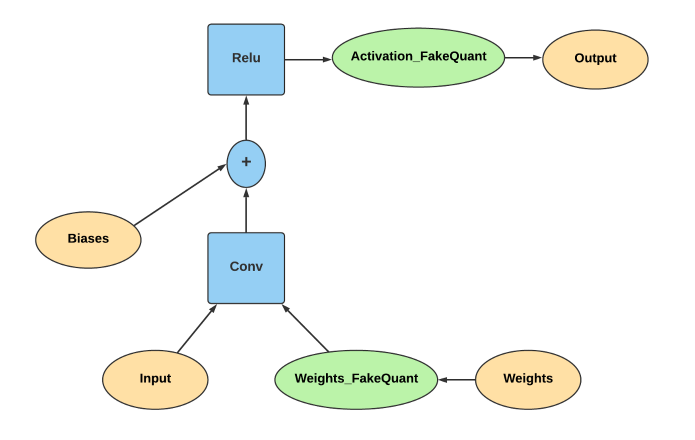
\includegraphics[width=\textwidth]{images/QAT.png}
    \caption{Quantization-aware Training. Duplicated from \cite{qunatifi}}
    \label{fig:myfigure}
\end{figure}
\\\\
Most of the edge TPUs supports only network compressed deep learning model, in order to accelerate the performance of neural network workloads. The popular compression technologies are quantization, pruning and knowledge distillation. Quantization is the process of lowering compute demand by converting 32-bit representation of parameter data into lower representations like 8-bit, 16-bit or others to make the model more compatible with edge device hardware architecture. This helps to achieve a reduced memory footprint, significantly reducing the number of transistors required in the chip. The three types of quantization methods are Quantization-aware Training(QAT), Post-Training Static Quantization(PTQ) and Post-Training Dynamic Quantization\cite{qunatifi}. QAT uses "fake quantized" nodes in forward \& backward passes to simulate the impact of lower bit representation during training and is more accurate than post training quantization methods.
\\\\
The deep learning based image processing tasks using edge devices is widely used in robotics, health care and manufacturing machine applications like quality inspection\cite{syberfeldt2020image}, metrology and packaging. However, there does not exist much work on uncertainty estimates for quantized deep learning models. This R\&D project investigates the impact of quantization with different uncertainty estimation methods and also deploy them on  edge devices.
\begin{figure}[h!]
    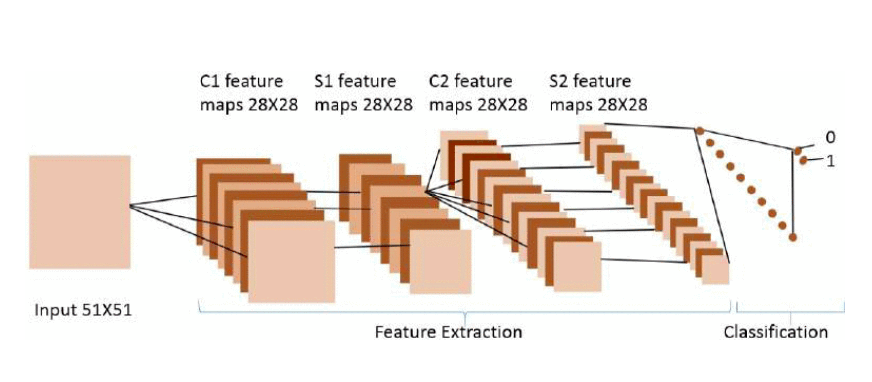
\includegraphics[width=\textwidth]{images/DNN.png}
    \caption{Deep neural network. Duplicated from \cite{DNN_Picture}}
    \label{fig:myfigure}
\end{figure}
\\\\
\textbf{Why is it important?} \\
Almost every industry is trying to boost automation for enhancing workflow, productivity, and safety with a range of tasks in unstructured world using edge AI. The deep learning model based inference engines deployed on edge devices makes decision for real-world problems. So it is important to study the uncertainty estimates for quantized model. This helps in the risk assessment for the decisions to be made for the model's prediction. The incorrect predictions of the model in safety-critical applications can endanger human lives. For instance, IBM's supercomputer Watson recommended 'incorrect and unsafe' cancer treatments\cite{ibm}. 
\\\\
One of the applications, uses a deep learning model to classify objects in the KUKA youBot\cite{bischoff2011kuka}, an omnidirectional mobile manipulator for education and research. The neural network workload is deployed on the robot controller hardware directly and due to its high computing demands, active perception is not possible. This robot is used in RoboCup@Work league\cite{kraetzschmar2014robocup} and one of the tasks is to pick a desired object from the multiple station environment. In one of the scenarios, the robot accidentally picked up the wrong object, due to wrong predictions made with high confidence. However, if the uncertainty score is calculated along with the model's prediction, a recovery action will be performed. And deploying this neural network workload in an edge device can help to perform active perception.
\\\\
As a result, it is important to evaluate differences in uncertainty estimates between quantized and non-quantized deep learning models. This study performs qualitative analysis of deep learning models deployed on edge devices, accelerating the growth of safety critical edge AI applications. 

\subsection{Problem Statement}
The rise in the popularity of edge computing throws new demands to computing platforms with regards to performance and energy efficiency. In safety critical and real world applications\cite{mcallister2017concrete}, the guarantees for decision making while using quantized deep learning model is vital and is required to evaluate the model uncertainty. The model must be aware of the fact that it will ultimately be quantized, so that it can perform all weight adjustments accordingly during training, to yield higher accurate predictions. QAT outperforms post training quantization methods and is used in this research.
\\\\
This R\&D aims to find and compare the probability distribution functions $f_{n}$, uncertainty in model predictions, where n $\in \mathbb{N}$, representing different uncertainty estimation methods. The function composes input data x and either non-quantized model parameters $\theta$ or quantized model parameters $\theta^{\prime}$. In order to evaluate the impact of quantization from the perspective of prediction reliability, the probability distribution functions $f_{1}(x, \theta)$ and $f_{1}(x, \theta^{\prime})$ are compared. In addition, this project compares the functions $f_{1}(x, \theta^{\prime})$, $f_{2}(x, \theta^{\prime})$, $f_{3}(x, \theta^{\prime})$.......$f_{n}(x, \theta^{\prime})$ to evaluate the uncertainty estimation methods for the quantized deep learning models.

% We assume that the that In terms of notation, y represents the prediction of the deep learning with x as the input data. The $\theta$ and $\theta^{\prime}$ represents the model parameters of the non-quantized and quantized deep learning models respectively. This R\&D work is to provide an empirical study on the uncertainty in the model predictions for non-quantized model y = f(x,$\theta$) and quantized model y = f(x,$\theta^{\prime}$). In addition, this research also focuses on using different uncertainty estimation methods for the quantized model and performs a comparative analysis among them.
% This R\&D work is to provide an empirical study of the uncertainty estimates for the quantized deep learning models from the perspective of edge computing.
% The rise in the popularity of edge computing throws new demands to computing platforms with regards to power, performance and energy efficiency. The success or failure of using edge devices for a specific task will ultimately depend on the right tradeoff among these metrics. In safety critical and real world applications such as risk assessment\cite{mackay1995bayesian}, autonomous driving\cite{mcallister2017concrete} and medicine\cite{liang2018bayesian}, the guarantees for decision making while using deep learning models is vital and is required to evaluate the model uncertainty for compressed neural networks. However, the recent research works evaluates the inference accelerators based on energy consumption for common inference workloads and inference time, which is not sufficient for safety intensive applications. Since quantization reduces model size while also enhancing training latency and inference, it is widely used in comparison with other model compression techniques\cite{rodriguez2018lower}. This R\&D work is to provide an empirical study of the uncertainty estimates for the quantized deep learning models from the perspective of edge computing.
% \\\\
% In terms of notation, we use D to donate data with n samples. The training and test data are represented by $D_{train}$ and $D_{test}$ respectively. The performance metric is related to the model uncertainty performance function tested with $D_{test}$, and represented by P(). The deep learning model before and after training with $D_{train}$ are represented by M($\theta$) and M($\theta^{\prime}$) respectively. The training can be performed with quantization techniques and the quantized trained deep learning model is represented via M($\theta^{\prime}_{q}$). 
% \\\\
% The performance metric of M($\theta^{\prime}_{q}$) is compared with M($\theta^{\prime}$) in this R\&D project.\
% P(M($\theta^{\prime}_{q}$)) ~~ P(M($\theta^{\prime}$))
\subsection{Research Questions}
What are the differences in uncertainty estimates of quantized deep learning models with different uncertainty estimation methods for classification, regression and segmentation tasks?
\begin{itemize}
    \item Taxonomy of uncertainty estimation methods in deep learning with special focus on single pass uncertainty estimation method
    \item Literature search on different quantization methods and which are supported by the DUT
    \item How does evidential loss function impact the QAT?
    % \item Which quantization methods are supported by the Device Under Test (DUT)?
    % \item How does the uncertainty estimates of quantized deep learning model differ from non-quantized deep learning model?
    % \item How does the uncertainty estimates of quantized deep learning model differ running on GPUs and edge devices?
\end{itemize}


\section{Related Work}
% \subsection{Survey of Related Work}
MLPerf\cite{reddi2019mlperf}, coalition of artificial intelligence accelerators from industry, academia and research labs, aiming to provide state-of-the-art performance evaluation for training and inference tasks. The internal structure of the MLPerf inference submission system has four components and are system under test(SUT), dataset, load generator(LoadGen), and an accuracy script. The LoadGen is a configuration file which handles the traffic generation, loading data for inference  and measuring performance. The query format created by LoadGen for different scenarios are single stream, multistream, server and offline. In single stream format, the next query is sent only after the completion of previous query. In multi stream format, the set of inferences per query is sent periodically with a  predefined time interval. In server format, the query is random and the SUT responds back within a defined latency limit. In offline format, the whole test data is sent as a batch and latency is not constrained. An empirical study to evaluate the system is performed by MLPerf with ResNet-50 v1.5 and MobileNet-v1 224 models on ImageNet dataset for classification task. The important contribution of this work is to identify the metrics and inference scenarios where AI accelerators are most useful.
\\\\
The most common benchmarking metrics of deep learning hardware accelerators are energy efficiency, performance and power\cite{libutti2020benchmarking} with their measurement terms: Operations per Watt, Time per inference, and Watt respectively. The aim of Domain Specific Architectures (DSA) is to accelerate inference related operations with reasonable power budget and the success or failure of these DSAs are determined by these benchmarking metrics in the state-of-the-art evaluations. 
\\\\
Achterhold et al. created a complex pruning and quantization strategy for pointwise NNs, but with the help of Bayesian inference\cite{achterhold2018variational}. The author trained a Bayesian neural network which is pruning \& quantisation friendly and with improper priors. They later converted it to pointwise NNs to achieve reduced memory, but the final non quantized Bayesian NNs were not able to estimate uncertainty because of improper priors\cite{ferianc2021effects}. This R\&D work is to learn a quantized NN directly and predicting model uncertainty considering a range of uncertainty estimation methods without changes in model architecture.

\section{Project Plan}
\subsection{Work Packages}
The R\&D project contains the following work packages
\begin{enumerate}
    \item[WP1] \textbf{Literature search}
        \begin{itemize}
        \item Taxonomy of neural network compression methods for deep learning model
        \item Literature search on quantization aware training for deep learning model
        \item Literature search on estimating uncertainty for deep learning models
        \item Literature search on uncertainty estimation evaluation methods
        \end{itemize}

    \item[WP2] \textbf{Experimental setup and analysis}
        \begin{itemize}
        \item Train ResNet\cite{he2016deep} DNN model with single pass uncertainty estimation methods for classification task on ImageNet\cite{russakovsky2015imagenet} dataset
        \item Perform experiments to estimate ResNet model uncertainty for classification task on GPU
        \item Train ResNet DNN model with quantization technique and single pass uncertainty estimation methods for classification task on ImageNet dataset
        \item Perform experiments to estimate quantized ResNet model uncertainty for classification task on GPU
        \item Comparative evaluation of the model uncertainty estimates for classification task between quantized and non-quantized deep learning models
        \end{itemize}
        
    \item[WP3] \textbf{Mid term report}
        \begin{itemize}
        \item Compile quantized ResNet model to support deploying on Google Coral - USB Accelerator and OAK-D with their respective compilers
        \item Perform experiments to estimate quantized ResNet model uncertainty for classification task on Google Coral - USB Accelerator and OAK-D devices
        \item Train MobileNet\cite{howard2017mobilenets} DNN model with quantization technique and single pass uncertainty estimation methods for classification task on ImageNet dataset
        \item Compile quantized MobileNet model to support deploying on Google Coral - USB Accelerator and OAK-D with their respective compilers
        \item Perform experiments to estimate quantized MobileNet model uncertainty for classification task on Google Coral - USB Accelerator and OAK-D devices
        \item Comparative evaluation of the model uncertainty estimates for difference in deep learning models, single pass uncertainty estimation methods and edge devices
        \end{itemize}
        
    \item[WP4] \textbf{Regression Task}
        \begin{itemize}
        \item Train ResNet DNN model with quantization technique and single pass uncertainty estimation methods on Facial Keypoints dataset
        \item Compile quantized ResNet model to support deploying on Google Coral - USB Accelerator and OAK-D with their respective compilers
        \item Perform experiments to estimate quantized ResNet model uncertainty for regression task on Google Coral - USB Accelerator and OAK-D devices
        \item Train MobileNet DNN model with quantization technique and single pass uncertainty estimation methods on Facial Keypoints dataset\cite{facialkey}
        \item Compile quantized MobileNet model to support deploying on Google Coral - USB Accelerator and OAK-D with their respective compilers
        \item Perform experiments to estimate quantized MobileNet model uncertainty for regression task on Google Coral - USB Accelerator and OAK-D devices
        \item Comparative evaluation of the model uncertainty estimates for difference in deep learning models, single pass uncertainty estimation methods and edge devices
        \end{itemize}
        
    \item[WP5] \textbf{Segmentation Task}
        \begin{itemize}
        \item Train ResNet DNN model with quantization technique and a single pass uncertainty estimation method on RoboCup@Work dataset \cite{robocupdataset}
        \item Compile quantized ResNet model to support deploying on Google Coral - USB Accelerator
        \item Perform experiments to estimate quantized ResNet model uncertainty for segmentation task on Google Coral - USB Accelerator device
        \end{itemize}
        
    \item[WP6] \textbf{Project report}
        \begin{itemize}
        \item Documentation of neural network compression techniques taxonomy for deep learning models
        \item Documentation of state-of-the-art uncertainty estimation methods for classification task
        \item Documentation of state-of-the-art uncertainty estimation evaluation methods
        \item Documentation of the quantization techniques support in the edge devices under test
        \item Documentation of uncertainty estimates for ResNet model with difference in tasks, dataset and uncertainty estimation methods
        \item Documentation of uncertainty estimates for MobileNet model with difference in tasks, dataset and uncertainty estimation methods
        \item Documentation of conclusions and recommendations for future work
        \item Draft R\&D report explaining research findings
        \item Final R\&D report explaining research findings
        \end{itemize}
\end{enumerate}

\subsection{Milestones}
    \begin{table}[H]
       \begin{tabular}{|m{0.35cm}|m{3cm}|m{10cm}|}
       \hline
       \textbf{M} & \textbf{Milestone} & \textbf{Checkpoints} \\
       \hline
       1 & Literature search & Taxonomy of NN compression methods. Read top research papers on uncertainty estimation for DL models\\
       \hline
       2 & Experimental setup & Train ResNet model and estimate uncertainty for classification task running on GPU\\
       \hline
       3 & Mid term report  &  Train quantized DNN models and estimate uncertainty for classification task running on edge devices\\
       \hline
       4 & Regression task & Train quantized DNN models and estimate uncertainty for regression task running on edge devices\\
       \hline
       5 & Segmentation task & Train quantized ResNet model and estimate uncertainty for segmentation task running on edge device\\
       \hline
       6 & Project report & Document all findings and submission of final report\\
       \hline
       \end{tabular}
        \caption{Project milestones}
        \label{tab:my_label}
    \end{table}


\subsection{Project Schedule}
\begin{figure}[h!]
    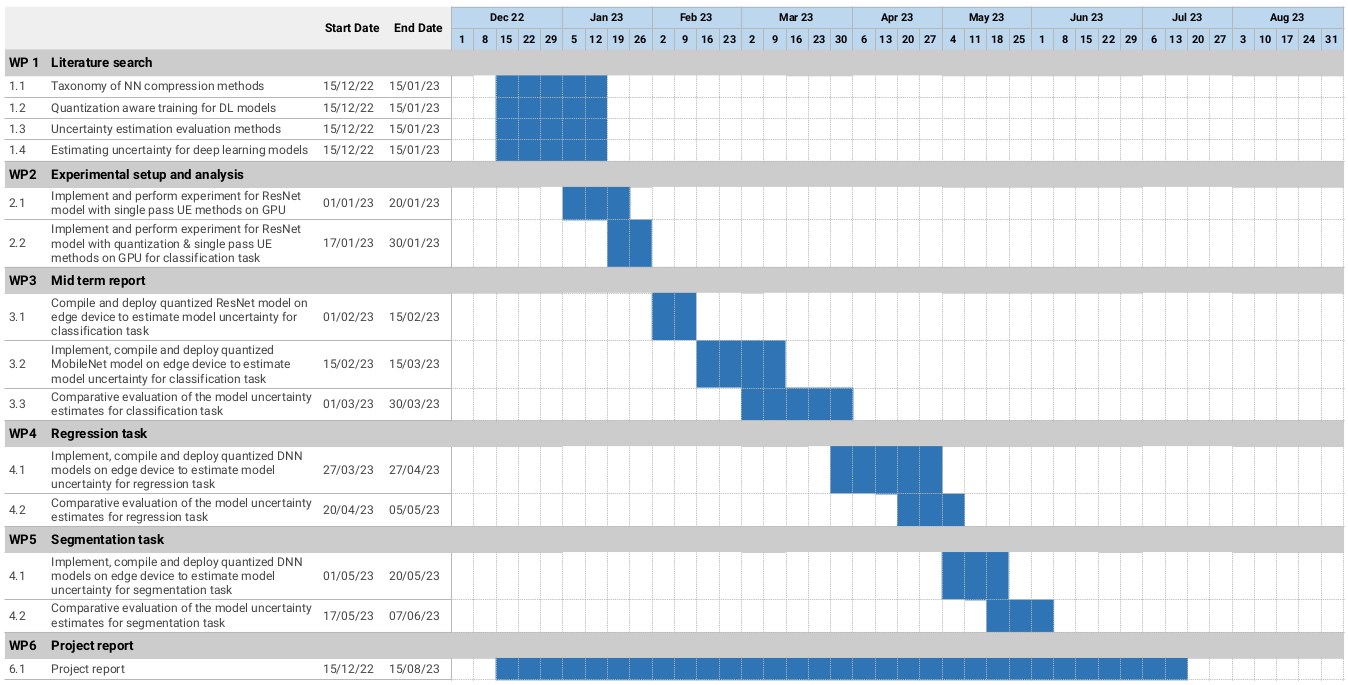
\includegraphics[width=\textwidth]{images/R&D Gantt Chart_V3.png}
    \caption{Project schedule}
    \label{fig:myfigure}
\end{figure}

\subsection{Deliverables}

\subsubsection*{Minimum Viable}
\begin{itemize}
    \item Taxonomy of neural network compression methods for deep learning model
    \item Train ResNet model with a single pass uncertainty estimation method on ImageNet dataset for classification task
    \item Perform experiments to estimate ResNet model uncertainty for classification task on GPU
    \item Train ResNet and MobileNet models with quantization techniques and single pass uncertainty estimation methods on ImageNet dataset for classification task
    \item Compile quantized ResNet and MobileNet model to support deploying on Google Coral - USB Accelerator and OAK-D
    \item Perform experiments to estimate quantized ResNet and MobileNet models uncertainty for classification task on Google Coral - USB Accelerator and OAK-D devices
    \item Comparative evaluation of the quantized model uncertainty estimates for classification task with difference in model, edge devices and single pass uncertainty estimation methods
\end{itemize}

\subsubsection*{Expected}
\begin{itemize}
    \item Train ResNet and MobileNet models with quantization techniques and single pass uncertainty estimation methods on Facial Keypoints dataset for regression task
    \item Compile quantized ResNet and MobileNet model to support deploying on Google Coral - USB Accelerator and OAK-D 
    \item Perform experiments to estimate quantized ResNet and MobileNet models uncertainty for regression task on Google Coral - USB Accelerator and OAK-D devices
    \item Comparative evaluation of the quantized model uncertainty estimates for regression task with difference in model, edge devices and single pass uncertainty estimation methods
    \end{itemize}

\subsubsection*{Desired}
\begin{itemize}
    \item Train ResNet model with quantization techniques and a single pass uncertainty estimation method on RoboCup@Work dataset for segmentation task
    \item Compile quantized ResNet model to support deploying on Google Coral - USB Accelerator
    \item Perform experiments to estimate quantized ResNet model uncertainty for segmentation task on Google Coral - USB Accelerator
    \item Evaluation of the quantized model uncertainty estimates for segmentation task
\end{itemize}

\newpage
% \nocite{*}
\bibliographystyle{plainnat} 
\bibliography{bibliography.bib}
\end{document}
